\subsection{Bausteinsicht}

Durch die hier folgenden Kapitel soll eine Übersicht über die implementierten Komponenten, ihre Funktionalität und ihre Verbindung zueinander gegeben werden.

Diese ist allerdings nur als abstrakte konzeptionelle Übersicht zu verstehen und stellt nicht die vollständige Realität dar.
Die Notwendigkeit ergibt sich, da für die tatsächliche Implementation 44 Komponenten mit insgesamt 212 TypeScript Quellcode-Dateien erstellt worden sind, die sich hier unmöglich alle darstellen lassen.

Zusätzlich zu diesen sind noch drei externe Pakete entstanden, die auf grund der Übersichtlichkeit hier ebenfalls ausgelassen worden sind.

Für einen vollständigen Überblick sollte das Git Code Repository aufgesucht werden.
Einen Verweis zu diesem ist in Kapitel \refsec{sec:artefacts} zu finden.

Die nachfolgenden Kapitel sind anhand der unterschiedlichen Arten von Komponenten im Kontext der Parallelität von JavaScript gruppiert.
Zusätzlich wird diese Klassifizierung auch für die Komponenten-Diagramme benutzt.

Diagramm-Boxen repräsentieren Runtimes oder Worker bzw. den Main-Thread der Runtime.
Diagramm-Komponenten können Applications, Realms oder Realm Componentes darstellen, festgestellt werden kann dies über den Kontext des Abschnittes.

Die Diagramm-Komponenten in einem Application Kapitel, stellen Realms dar, in einem Realm Kapitel sind es dann wiederrum Realm Components und in einem Realm Components Kapitel können sie Dateien oder Klassen sein.

Das bedeutet auch, dass die Namen der Diagramm-Komponente aus den Application Kapiteln in Realm Kapiteln und die aus den Realm Kapiteln in Realm-Component Kapiteln beschrieben werden und durch sie assoziiert werden.

\subsubsection{Client Server Architektur}
\label{sec:client-server-arch}

Wie bereits in der Lösungsstrategie beschrieben, soll diese Anwendung als Client Server Anwendung realisiert werden.
Dadurch unterteilt sich diese Anwendung in zwei übergeordnete Komponenten.


\begin{figure}[htb]
    \centering
    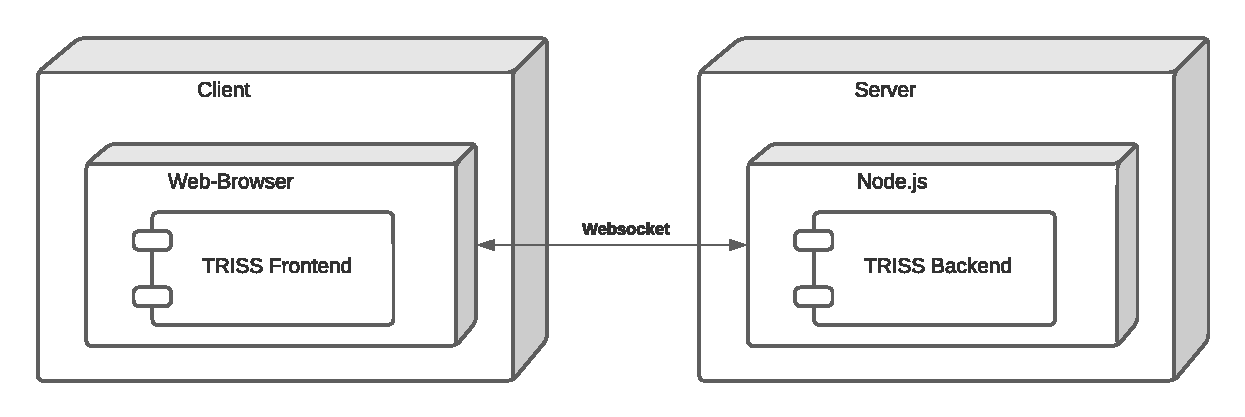
\includegraphics[scale=.65,center]{medien/client-server-start.pdf}
    \caption{Abstrakte Client Server Architektur}
    \ownsource
    \label{fig:abstract-client-server}
\end{figure}

\FloatBarrier

Der Client ist dabei das physikalische System, mit dem der Nutzer interagiert.
Auf diesem System muss ein moderner Webbrowser installiert sein, mit dem er das \highlight{TRISS Frontend} bezieht.
Das Frontend stellt dem Nutzer die Möglichkeit bereit, Server-Entitäten anzulegen und einzusehen.
Ebenfalls erlaubt er es, das Layout bzw. die Instanz via einer 3D-Darstellung zu erstellen und einzusehen.
Das Frontend Artefakt wird dabei durch einen statischen HTTP-Server bereitgestellt.

Das zweite Artefakt, das über den Server bereitgestellt wird, ist das \highlight{TRISS Backend}, das alle dynamischen Aktionen des Clients ermöglicht und gleichzeitig die Simulation bereitstellt.

Das Backend wird dabei im Gegensatz zu dem Frontend nicht via HTTP, sondern über das WebSocket-Protokoll angesprochen.
Der Vorteil besteht darin, dass dadurch das Backend nicht nur angesprochen werden kann, sondern auch Nachrichten ohne Anfrage an den Client senden kann.
Zusätzlich kommt die WebSocket-Verbindung, im Gegensatz zu HTTP oder Long-Polling\footnote{\url{https://javascript.info/long-polling}}, mit nur einer permanenten TCP-Verbindung aus\footnote{\url{https://datatracker.ietf.org/doc/html/rfc6455\#section-1.1}}.
Das reduziert nicht nur die Roundtrip-Zeit, sondern senkt auch zusätzlich den Berechnungs-Overhead, kontinuierlich neue TCP-Verbindungen aufzubauen.

Eine relevante Eigenschaft dieser Architektur ist, dass der Nutzer außer einem modernen Webbrowser keine weitere Software auf dem Gerät installiert haben muss, mit dem er die Anwendung verwalten will.
Es müssen nur das \highlight{TRISS Frontend} und das \highlight{TRISS Backend} vorher auf einem Server installiert worden sein.

Um die Inbetriebnahme weiter zu vereinfachen, werden beide Server Artefakte bzw. deren respektive Runtimes in zwei Docker Container verpackt.
Diesbezüglich folgen genauere Informationen im Kapitel \refsec{sec:distribution-view}.

\subsubsection{Application – TRISS Backend}
\label{sec:triss-backend-component}

Das TRISS Backend ist in drei Realms aufgeteilt.
Die zentrale Komponente ist die \highlight{Backend Server} Komponente, die als Single Source of Truth agiert und eingehende WebSocket-Verbindungen annimmt, Instanzen erstellt, deren Zustand verwaltet, die Erstellung von Agenten und Layouts erledigt und Frames zum Client schickt.

Allerdings produziert sie keine neuen Frames oder betreibt die Simulation, das erledigt die zweite Komponente, die \highlight{Worker Simulation Instance}.
Diese hat ein vergleichbar einfaches Interface, über das man die Welt und den Agenten setzen, die aktuelle Fahrzeugposition abfragen und die Simulation einen Schritt weiter laufen lassen kann.

Die dritte Komponente ist die \highlight{Worker Agent Sandbox} welche vom Backend Server dafür verwendet wird, um die Syntax und Interface Korrektheit eines neu erstellten Agenten zu prüfen.

Diese klare Aufteilung der Funktionen erlaubt es dann die \highlight{Worker Simulation Instance} als eigenen Worker auszuführen.
Dies wiederum hat einige Vorteile.
Der zentrale Vorteil ist, dass der Worker eine echte parallele Ausführung der Komponenten erlaubt und es somit möglich macht, eine Multicore CPU effizient zu verwenden.
Zusätzlich dazu, ist der Worker vom Server isoliert, wodurch der Agent schwerer den Server abstürzen lassen kann.
Auch kann der Worker so eigene globale Bibliotheken importieren und verwenden, ohne darauf achten zu müssen, dass diese nicht mit anderen Agenten oder dem Server kollidieren.

\begin{figure}[htb]
    \centering
    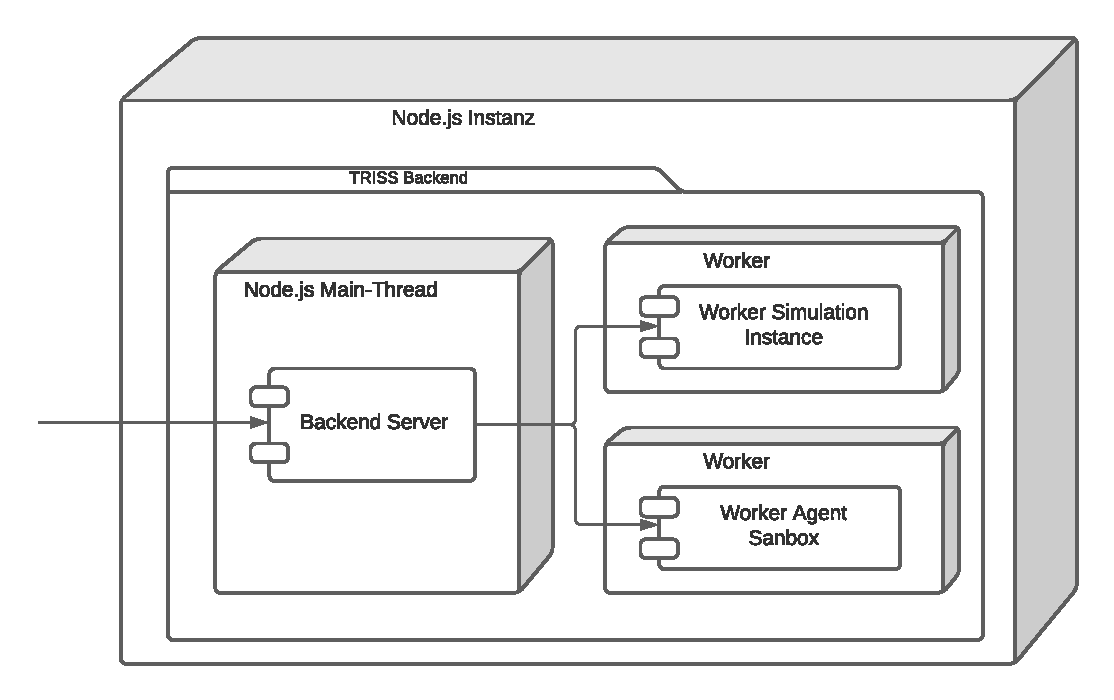
\includegraphics[scale=.65,center]{medien/triss-backend.pdf}
    \caption{Abstrakter Backend Server}
    \ownsource
    \label{fig:triss-backend}
\end{figure}

\FloatBarrier

Wie bereits beschrieben, hat JavaScript keine klassischen Threads, welche auf die gleichen Objekte zugreifen können.
Dieser Aspekt ist für diese Anwendung sehr relevant.
Denn damit ist die Isolation zwischen zwei Realms programmiertechnisch identisch zu der zwischen dem Node.js Server und der JavaScript Runtime des Browsers.
Das erlaubt es, alle Übertragungen gleichartig durchzuführen, ohne dabei unnötig Performance-Einbußen in Kauf zu nehmen.

Zusätzlich lassen sich die Komponenten identisch ansprechen, egal ob sie nun auf dem gleichen physischen System betrieben werden oder nicht.
Das bedeutet auch, dass sich der Server ohne größeren Auffand so erweitern lässt, dass er in einem Hardware-Cluster die Rechenlast verteilen könnte.
Es könnten aber auch beispielweise Agenten in einem Worker der Browser JavaScript Runtime ausgeführt werden, wenn dieser nicht Node.js spezifische Bibliotheken bzw. Schnittstellen braucht.

Dies bringt einen weiteren Vorteil mit sich, der hier ausgenutzt wird.
Dadurch kann nämlich der gleiche Serialisierungs-Algorithmus für alle Realm Übergänge verwendet werden sei es nun vom Backend Server zum Worker, vom Backend zum Frontend oder auch vom Backend zum Massenspeicher.
Dadurch ergibt sich ein weiterer sehr bedeutender Vorteil, so können Daten \enquote{getunnelt} werden, was hier durch die Worker bzw. durch den Backend Serve angewendet wird.

Wenn die Worker einen Frame, also einen diskreten Zustand, erzeugt haben, serialisieren sie diesen, mit dem Frame Serializer und schicken die Daten verpackt in ein Message Objekt an den Server.
Dieser packt das Message-Objekt aus, deserialisiert allerdings den Frame nicht, sondern verpackt diesen nur erneut in ein anderes Message-Objekt, das er an den Client schickt.
Dieser deserialisiert das vollständige Message-Objekt samt dem enthaltenen Frame und kann dann dort auf die hinterlegten Fahrzeuge zugreifen.

Für diese Aufgabe wurde im Kontext der Projektarbeit eine Bibliothek entwickelt, die vorgegebene Datenstrukturen in ein Binärformat um- und zurück wandelt.
Dieses Paket wurde \textit{serialization-generator}\footnote{\url{https://www.npmjs.com/package/serialization-generator}} genannt und via npm öffentlich zur Verfügung gestellt.
Auch wenn es andere Lösungen zur Serialisierung gegeben hätte, ist diese besonders an diese Verwendung angepasst, insofern sie auf die Benutzung mit TypeScript mit statischen Datenmodellen optimiert ist.

\subsubsection{Realm – Backend Server}

Der Backend Server ist die zentrale Komponente des TRISS-Backends.
Ihre Hauptaufgabe besteht darin, Verbindungen und Entitäten zu verwalten.

Zu diesen Verbindungen zählen die zu den Frontend Clients und den Worker Simulation Instances.
Die Menge der Entitäten enthält vor allem solche, die die Welt, den Agenten oder den aktuellen Simulationszustand in Form von Fahrzeugen repräsentieren.

\begin{figure}[htb]
    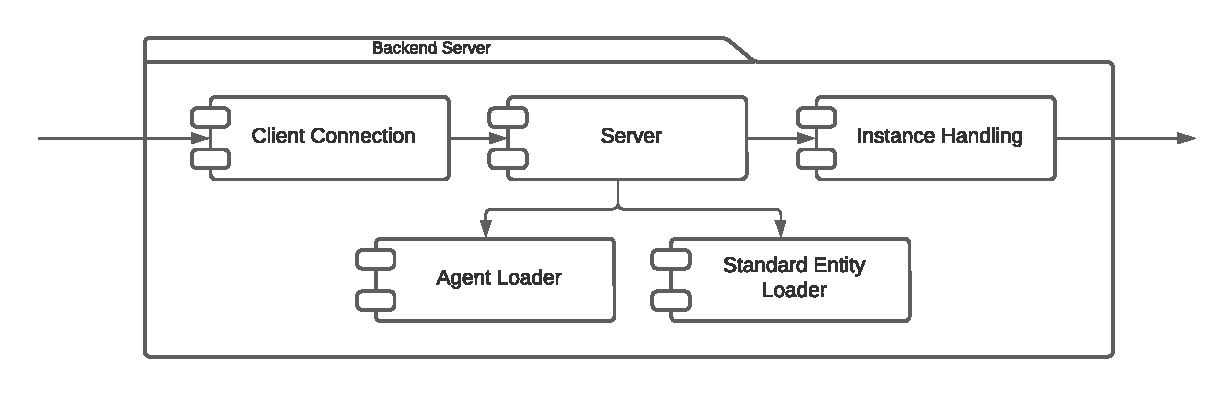
\includegraphics[scale=.65,center=\linewidth]{medien/backend-server.pdf}
    \caption{Backend Server}
    \ownsource
    \label{fig:backend-server}
\end{figure}

\FloatBarrier

Der Backend-Server ist der Realm, der alle Programmbestandteile zusammenbringt, Nachrichtenaustausch ermöglicht und Worker verwaltet.
Er leitet Nachrichten an die Clients weiter und ermöglicht Operationen auf den Entitäten auszuführen.

Dafür teilt er sich in fünf Komponenten, wobei alle bis auf den Server für die Kommunikations-Herstellung bzw. Entitäts-Bereitsstellung verantwortlich sind, und der Server diese nur verwaltet.
Dies repräsentiert sehr deutlich die Aufgabe dieses Realms.

\subsubsection{Realm – Worker Simulation Instance}

Der Worker Simulation Instance Realm beinhaltet die eigentliche Simulation und betreibt den dazugehörigen Agenten.
Um diese zu erledigen, besteht er aus drei Paketen.

\begin{figure}[htb]
    \centering
    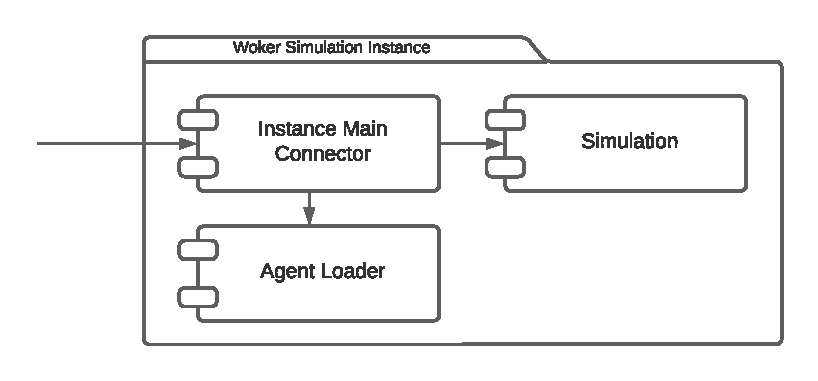
\includegraphics[scale=.65,center]{medien/worker-simulation-instance.pdf}
    \caption{Worker Simulation Instance}
    \ownsource
    \label{fig:worker-simulation-instance}
\end{figure}

\FloatBarrier

Der Realm ist insgesamt relative einfach gehalten und besitz ein kleines Interface um die Welt und die Agenten ID entgegenzunehmen, und diese dann weiterzuleiten bzw. zu laden und dann in Betrieb zu nehmen.

Die Worker Simulation Instance Komponente repräsentiert immer genau eine Simulationsinstanz und bleibt für die Komplette dauer der Lebenszeit der Instanz bestehen.

Sie wird durch Nachrichten gesteuert und übersetzt diese auf die Simulation.
Im Gegensatz zum Backend Server Realm hat sie eine bedeutend höhere CPU Auslastung, da sie nicht nur durch den Agenten die eigentliche Simulation errechnet, sondern auch die Frames serialisiert.

\subsubsection{Realm – Worker Agent Sandbox}

Die Sandbox wird dafür eingesetzt, neu erstellte Agenten, die vom Frontend empfangen worden sind, auf Syntax-Korrektheit und auf ihre Interface-Konformität zu prüfen.

Dies geschieht in einem eigenen Realm, damit bei Syntaxfehlern nicht der gesamte Server abstürzt.

\begin{figure}[htb]
    \centering
    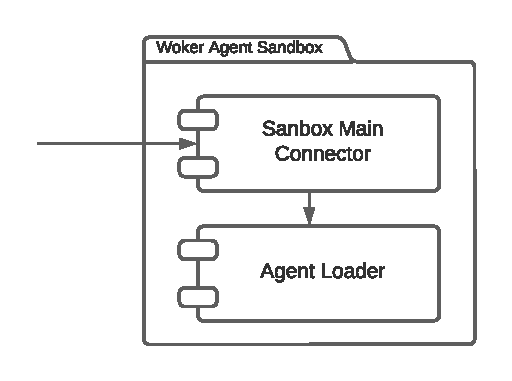
\includegraphics[scale=.65,center]{medien/worker-agent-sandbox.pdf}
    \caption{Worker Agent Sandbox}
    \ownsource
    \label{fig:worker-agent-sandbox}
\end{figure}

\FloatBarrier

Dafür benötigt er ebenfalls den Agent Loader, den er nach der Initialisierungsnachricht direkt verwende um den Agenten Testweise zu laden und so direkt prüfen zu können, ob das Laden erfolgreich ist, also alle Importpfade korrekt sind und die Syntax des JavaScript-Codes korrekt ist.

Wenn das gelungen ist, prüft er, ob alle Schnittstellen implementiert worden sind und liefert das Resultat wieder an den Main-Thread zurück.
Daraufhin wird er von außen wieder heruntergefahren.

\subsubsection{Realm Component – Server}

Die Server Komponente ist für den Backend Server Realm die verwaltende Kraft, alle anderen werden entweder von ihr angesprochen oder sprechen diese an.

\begin{figure}[htb]
    \centering
    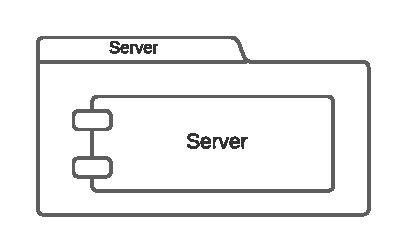
\includegraphics[scale=.65,center]{medien/server.pdf}
    \caption{Server}
    \ownsource
    \label{fig:server}
\end{figure}

\FloatBarrier

Sie verwaltet die Simulations-Instanzen, die Agenten und die Entitäten.
Diese Komponente wird bei der Ausführung des Servers als Singleton erstellt und bleibt bis zum Ende der Ausführung bestehen.

\subsubsection{Realm Component – Agent Loader}

Der Agent Loader ist von besonderer Bedeutung für den Server.
Er erlaubt es neue Agenten anzulegen und sie zu verwalten.

\begin{figure}[htb]
    \centering
    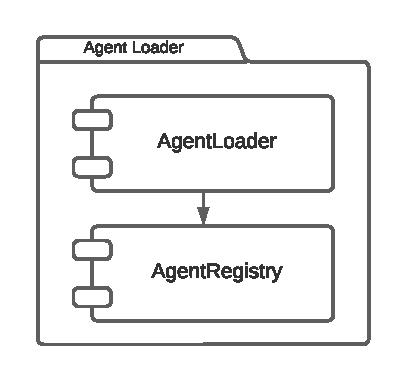
\includegraphics[scale=.65,center]{medien/agent-loader.pdf}
    \caption{Agent Loader}
    \ownsource
    \label{fig:agent-loader}
\end{figure}

\FloatBarrier

Durch die bereits aufgezeigte Eigenschaft, dass Realms vollständig voneinander getrennt sind, wird sie vor allem dafür eingesetzt, um den Agenten in dem Backend Server Realm zu speichern und dann im Worker Agent Sandbox und Worker Simulation Instance Realm wieder zu laden.
Deshalb muss sie gespiegelt in allen Realms des TRISS Backends erzeugt werden, jedoch werden jeweils unterschiedliche Funktionen von ihr verwendet.

Für die Bereitstellung hält er intern ein Register, was es ihm erlaubt Anfragen bezüglich der Liste von Agenten direkt zu beantworten, anstatt auf den Massenspeicher zugreifen zu müssen.

Nach dem Speichern liefert er eine ID zurück, welche dann vom Server verwendet wird, um auf diesen Agenten zu verweisen.

Geladen werden die JavaScript Sourcecode-Dateien über das ES-Module-System, als dynamischer import.
Dies erlaubt eine robuste und spezifikationskonforme Verwaltung und macht die Verwendung bzw. Implementation für den Nutzer vorhersehbarer und einfacher.

\subsubsection{Realm Component – Client Connection}

Die Client Connection Komponente bündelt alle Aspekte welche benötigt werden, damit der Client mit dem Server über das WebSocket Protokoll interagieren kann.

Eine der ersten Komponenten, die der Server dafür instanziiert, ist die WebSocket Server Klasse, die dann über den beigefügten TCP-Port auf neue Verbindungen wartet und dann, sollte er eine empfangen, eine Individual WebSocket Handler Komponente dafür erzeugt.

\begin{figure}[htb]
    \centering
    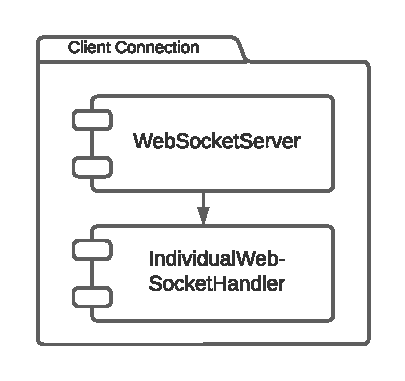
\includegraphics[scale=.65,center]{medien/client-connection.pdf}
    \caption{Client Connection}
    \ownsource
    \label{fig:client-connection}
\end{figure}

\FloatBarrier

Diese Komponente repräsentiert den individuellen Zustand der Client-Ver\-bindung, wie zum Beispiel welche aktuelle Instanz betrachtet wird.
Sie ordnet zentral die Anfrage-Nachrichten entsprechende Methoden Aufrufe zu und erzeugt die dazugehörigen Antwort-Nachrichten.

\subsubsection{Realm Component – Instance Handler}

\begin{figure}[htb]
    \centering
    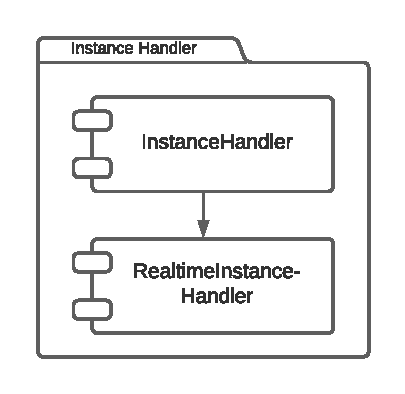
\includegraphics[scale=.65,center]{medien/instance-handler.pdf}
    \caption{Instance Handler}
    \ownsource
    \label{fig:instance-handler}
\end{figure}

\FloatBarrier

Der Simulation Instance Realtime Handler, ist die Komponente, die die Worker Simulation Instance Komponente verwaltet und als Repräsentant im Backend Server dafür einsteht.
Sie agiert ähnlich zu der Individual Web Socket Handler Komponente und übersetzt Methoden-Aufrufe zu Message-Objekten, die sie serialisiert und überträgt.
Zusätzlich beinhaltet sie Caches, damit beispielweise mehrere Individual WebSocket Handler auf den aktuellen Frame zugreifen können.

\subsubsection{Realm Component – Standard Entity Loader}

Der Standard Entity Loader wird vom Backend Server verwendet um dem Nutzer direkt eine kleine Auswahl an vorbereiteten Layouts und Agenten zur Verfügung zu stellen.

\begin{figure}[htb]
    \centering
    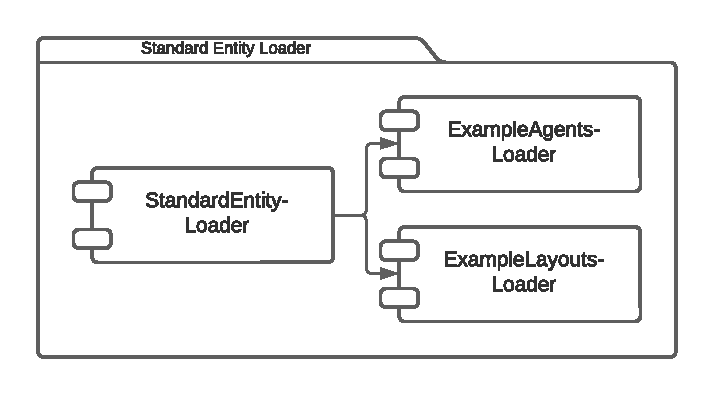
\includegraphics[scale=.65,center]{medien/standard-entity-loader.pdf}
    \caption{Standard Entity Loader}
    \ownsource
    \label{fig:standard-entity-loader}
\end{figure}

\FloatBarrier

Dafür wurden die Komponente so konfiguriert, dass sie eine statische Liste mit Einträgen laden und an den Server zur Registrierung übermittelt.

Besonders wichtig ist dabei das Laden des Random Exit Drivers, der als Beispiel Agent viele Aspekte für die Implementierung eines solchen demonstriert.

Die Standard-Layouts umfassen von einfachen manuell erstellen Layouts, welche die besonders groß sind, viele Routen zulassen, viele Kreuzungen beinhalten, viele Erzeugungs- und Zerstörungs-Punkte beinhalten und eines das Leer ist.

Diese sollen dabei unterstützen noch schneller mit der Entwicklung und dem Experimentieren beginnen zu können.
Zusätzlich können sie als Beispiel für die Entwicklung von komplizierteren Layouts benutzt werden und deren Implementationen inspirieren.

So wurde beispielweise ein auf dem Wave-Function-Collapse-Algorith-\linebreak mus\autocite{wfca2019} basierter Layout Generator erstellt, welcher ein guter Startpunkt sein kann, um eine organischeres Layout in der Größenordnung einer kleineren Ortschaft zu erzeugen.

\subsubsection{Realm Component – Simulation}

Die eigentliche Simulation besteht aus zwei Komponenten, die unabhängig vom Kontext, also ob sie nun von einem Worker verwendet werden oder nicht, so angesprochen werden sollten.
Dabei nimmt die Simulation Instance die verwaltende und kapselnde Rolle bezüglich der Simulation ein und abstrahiert welche Engine verwendet wird und wie diese konkret angesprochen wird.
Sie beinhaltet auch Meta-Informationen, wie beispielweise den Namen oder die ID der Simulation.

\begin{figure}[htb]
    \centering
    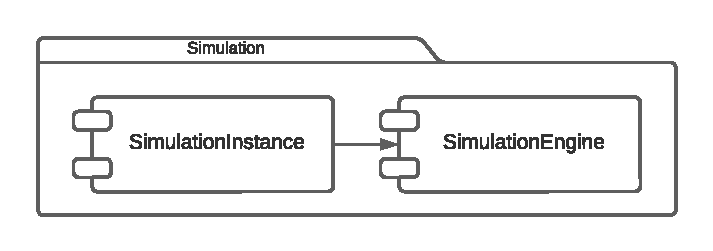
\includegraphics[scale=.65,center]{medien/simulation.pdf}
    \caption{Simulation}
    \ownsource
    \label{fig:simulation}
\end{figure}

\FloatBarrier

Die Engine ist das eigentliche ‚Herzstück‘, das die Simulation an sich vorantreibt.
Sie erhält über die Simulation Instance von dem Instance Main Connector den Agenten, den sie verwenden soll, um die Simulation zu betreiben.
Sie verwaltet intern alle notwendigen Zustände und spricht den Agenten mit diesen an.
Für den Agenten stellt sie die Schnittstelle zu dem restlichen System dar, insofern sie die einzige Referenz ist, die an den Agenten übergeben wird.

Hier bestünde die Möglichkeit, die Software zu erweitern, in dem andere Varianten der Engine entwickelt werden.
Diese könnte dann beispielweise eine andere Art von Agenten unterstützen, welcher lokal auf nur einem Fahrzeug agiert und dadurch direkt von der Engine multithreaded werden könnte.
Eine weitere Option wäre eine Engine, die andere Prozessschritte inkludiert, wie beispielweise eine Kollisionsberechnung als Validierungsschritt.

\subsubsection{Realm Component – Instance Main Connector}

\begin{figure}[htb]
    \centering
    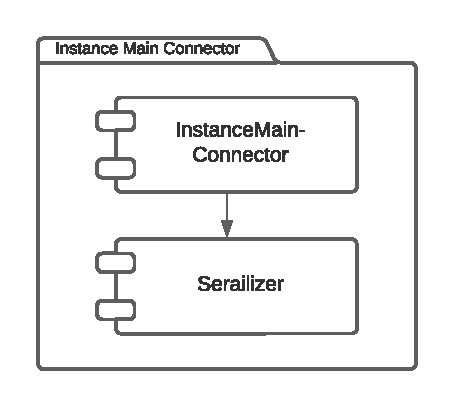
\includegraphics[scale=.65,center]{medien/instance-main-connector.pdf}
    \caption{Instance Main Connector}
    \ownsource
    \label{fig:instance-main-connector}
\end{figure}

\FloatBarrier

Das Instance Main Connector Paket stellt die Abstraktion bezüglich der Verwendung in einem Worker bereit und erlaubt die Verwendung der Simulation in dieser Konstellation.
Er stellt das Gegenstück zu dem Simulation Instance Realtime Handler aus dem Backend Server dar und tauscht mit diesem Nachrichten aus.
Er ist die einzige semantische Verbindung zum Gesamtsystem.

Er verwendet wie auch die anderen Realm-Übergänge die entsprechenden Serialisierer.


\subsubsection{Realm Component – Sandbox Main Connector}

Diese Komponente hat die gleiche Rolle wie der Instance Main Connector, nur für die Sandbox.

\begin{figure}[htb]
    \centering
    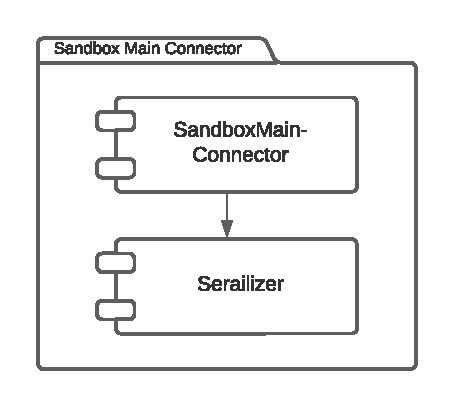
\includegraphics[scale=.65,center]{medien/sandbox-main-connector.pdf}
    \caption{Sandbox Main Connector}
    \ownsource
    \label{fig:sandbox-main-connector}
\end{figure}

\FloatBarrier

Im Gegensatz zu ihr, besitzt dieser jedoch andere Kommandos und verwendet selbst andere Komponenten.
Zusätzlich ist er anders gegen Fehler geschützt und liefert diese zurück an den Main-Thread, damit dieser diese Fehlermeldung wiederum an den Client geben kann und somit der Nutzer nachvollziehen kann, warum der Agent ggf. abgelehnt worden ist.

\subsubsection{Application – TRISS Frontend}
\label{sec:triss-frontend-component}

Das TRISS Frontend ist das zweite eigenständige Element der TRISS Anwendung.
Sie ist ein rein passives Element und enthält keine Anwendungslogik, sondern dient lediglich der Ansteuerung der Anwendung und Visualisierung der Simulation.

\begin{figure}[htb]
    \centering
    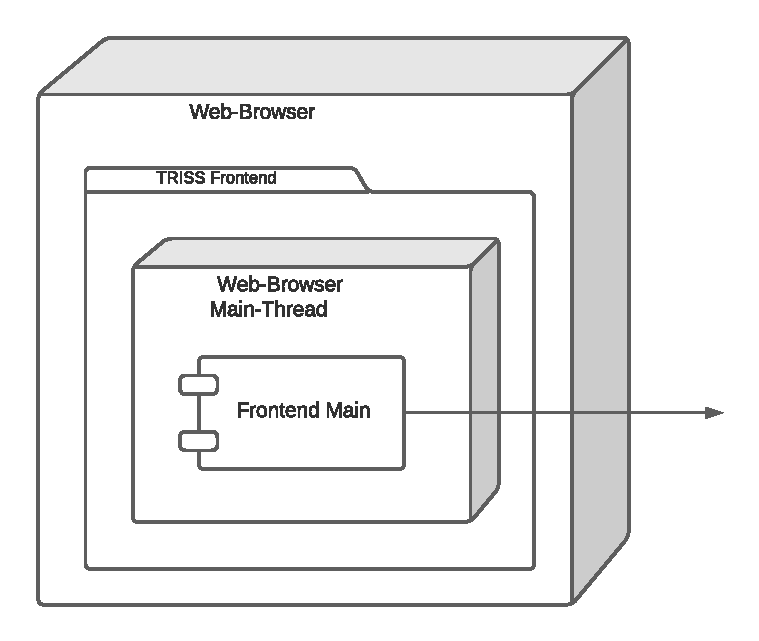
\includegraphics[scale=.65,center]{medien/triss-frontend.pdf}
    \caption{TRISS Frontend}
    \ownsource
    \label{fig:triss-frontend}
\end{figure}

\FloatBarrier

Sie besteht aus einem einzigen Realm, welcher die komplette Anwendung umschließt.
Neben dem JavaScript Realm betreibt das Frontend, wie im weiteren Verlauf erläutert, durch three.js eine WebGL Kontext, der hier jedoch nicht mit eingezeichnet ist.

\subsubsection{Realm – Frontend Main}

Der Frontend Main Realm, ist sehr umfangreich und teilt sie sich in vier Hauptkomponenten.

\begin{figure}[htb]
    \centering
    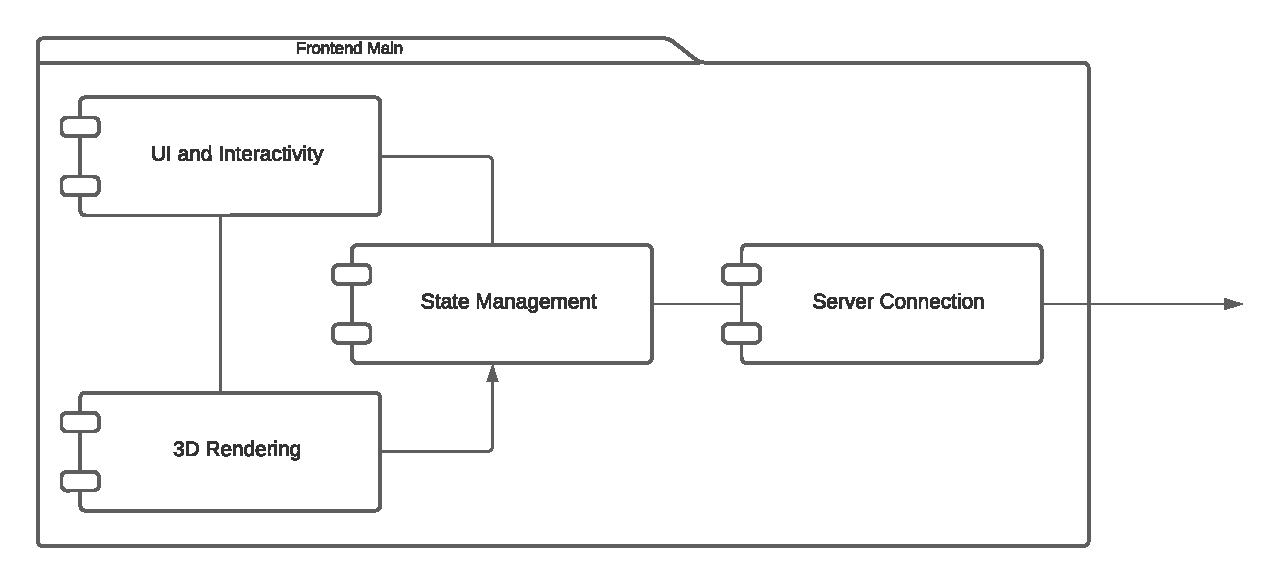
\includegraphics[scale=.65,center]{medien/frontend-main.pdf}
    \caption{Frontend Main}
    \ownsource
    \label{fig:frontend-main}
\end{figure}

Das zentrale Element dabei ist die State Management Komponente.
Sie vereint alle Aspekte rund um die Spiegelung der Server-Status als auch die Speicherung des UI-Zustands.
Sie dient als Single Source of Truth bzw. dessen Spiegelung.
Mit bzw. über diese Komponente kommunizieren alle anderen.
Es wurde versucht, die Anwendung so zu entwickeln, dass alle anderen Komponenten zustandslos sind.

Die Server Connection Komponente ist dabei der Counterpart der Individual WebSocket Connection Komponente und vereint ähnlich wie diese die De-/Serialisierung und das Abbilden von Methoden auf Nachrichten und umgekehrt.
Darüber hinaus ist sie auch dafür zuständig vom, HTTP-Server die Assets zu laden, da dies programmatisch und nicht vom Browser gesteuert wird.
Sie gibt alle erhaltenen Informationen an das State Management weiter und wird durch dieses bzw. dessen Events beauftragt, Daten einzuholen.

UI and Interactivity umfasst all die Aspekte des Frontends, mit denen der Nutzer interagieren und welche er sehen kann.
Sie stellt den Zustand dar, welchen das State Management aktuell hat, und meldet Ereignisse an dieses.
Diese Komponente befindet sich in einer Koexistenz mit dem 3D-Rendering, das auf Grundlage seiner Komplexität nicht mehr Teil der UI ist.
Diese Komponente bettet das 3D Rendering ein, liefert ihm den UI-Kontext und verarbeitet Events.

Die letzte, jedoch sehr zentrale Komponente, ist die 3D-Rendering-Kompo\-nente.
Diese umfasst, wie der Name andeutet, alle Aspekte bezüglich der drei dimensionalen Darstellung der Welt.
Sie ist als eine einzelne Komponente gefasst, da sie nur auf dem Parameter Welt beruht und somit ohne weiteres anderweitig verwendet werden könnte.
Des Weiteren ist sie bedeutend komplizierter und anders in ihrer Programmierung als die UI.

Die 3D-Rendering-Komponente ist, genauso wie die Datenübertragung und die Agenten, eine der Flaschenhälse, da sie direkt und in Abhängigkeit zur Menge der Fahrzeuge die Performance beeinflusst.
Deshalb wurde hier besonders auf die Implementation und deren Laufzeitverhalten Wert gelegt.

\FloatBarrier

\subsubsection{Realm Component – State Management}

Die Frontend Anwendung beruht zentral auf der Verwaltung des UI Zustandes.
Die größte Herausforderung, die bei der Entwicklung von Frontend Anwendungen anzutreffen ist, ist die Verwaltung des Zustandes der UI, der fachlichen Informationen und des Server Zustands.
Die Herausforderung tritt vor allem dann zutage, wenn versucht wird bei einer Frontend Anwendung Fehler zu finden, welche keinen Schwerpunkt auf die Zustandsverwaltung gelegt hat.
Diese Verwaltung hat demzufolge einen hohen Stellenwert erhalten und wurde in diesem Kontext zentral behandelt.

\begin{figure}[htb]
    \centering
    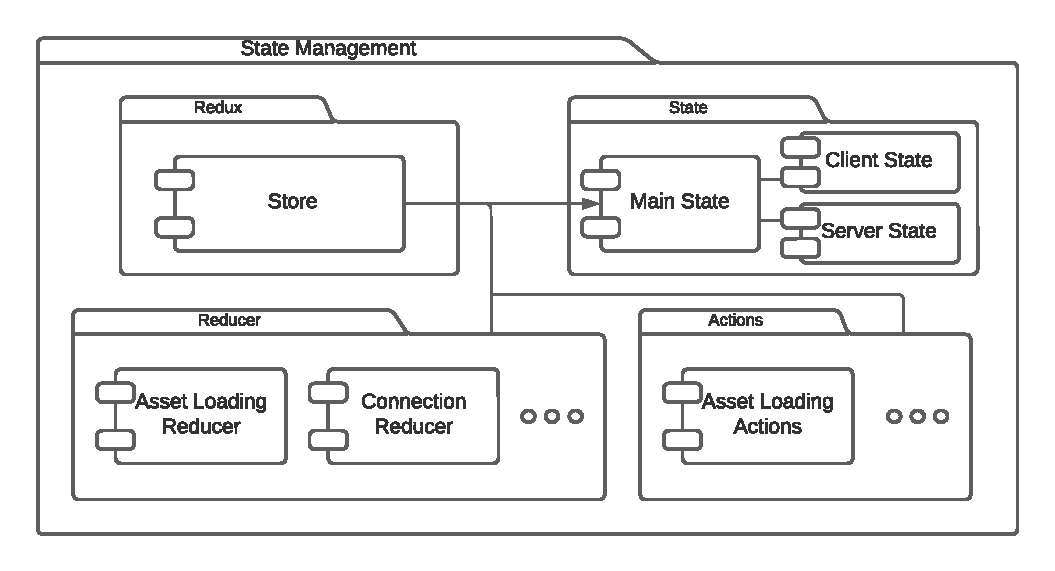
\includegraphics[scale=.65,center]{medien/state-management.pdf}
    \caption{State Management}
    \ownsource
    \label{fig:state-management}
\end{figure}

% \FloatBarrier

Da diese Aufgabe so zentral und typisch für das Frontend ist, bestehen dafür auch Standardlösungen.
Für diese Anwendung wurde sich für eine der am \helptex häufigsten verwendeten Lösungen\footnote{\url{https://2020.stateofjs.com/en-US/technologies/datalayer/\#datalayer_experience_ranking} (Es muss auf den \enquote{Usage} Reiter geklickt werden.)} entschieden, Redux.

Redux wird in dieser Anwendung als die zentrale Instanz für die Zustandsverwaltung verwendet.
Es handelt sich hierbei um eine verhältnismäßig einfache Bibliothek, die eher als Programmierkonzept anstatt als eine hoch komplexe technische Lösung angesehen werden sollte.
Es schreibt gewisse Verhaltensweisen bezüglich der Zustandsverwaltung vor, die, wenn man sie einhält, den Code bedeutend einfacher macht, viele Fehler vermeidet und es einem erlaubt die Anwendung bzw. deren Zustand über Werkzeuge zu analysieren und Fehler zu finden.

Diese Konzepte, die Redux vorschreibt, beziehen sich dabei konkret auf drei Arten von Komponenten, in die auch diese State Management Komponente aufgeteilt ist.
Das erste, das auch initial definiert werden muss, ist der Zustand der hier im Paket State enthalten ist.
Dabei handelt es sich um die Definition eines Objekt-Baumes, der für TRISS mit einem Main State als Wurzelknoten beginnt und dann den Client und den Server State beinhaltet.
Der Client State ist dabei der UI State und der Server State umfasst alle gespiegelten Daten vom Server, wie beispielweise welche Instanzen zur Verfügung stehen und welchen Frame als letztes von einer dieser erhalten worden ist.

Dieser Zustand wird von dem Redux Store gespeichert und verwaltet.
Der Zustand gilt als unveränderlich und wird nicht angepasst, sondern ersetzt, was im Kontext von JavaScript viele Fehler im Vorhinein verhindert und bedeutende Debugging-Möglichkeiten erschafft.
Um diesen Zustand zu ersetzen bedarf es sogenannte Reducer, die den aktuellen Zustand und die Action (ein Ereignis des Systems) als Parameter entgegen nehmen.
Aus diesen beiden Informationen erzeugt diese pure function\footnote{\url{https://en.wikipedia.org/wiki/Pure_function}} dann einen neuen Zustand, der den vorangegangenen ersetzt.

Diese Reducer enthalten also die UI bzw. Anwendungslogik.
Dadurch, dass sie pure sein müssen, der initiale Zustand bekannt ist und alle Events einfache Objekte sind, die man aufzeichnen kann, kann genau nachvollzogen werden, was zu dem aktuellen Anwendungszustand geführt hat.
Es lassen sich die Events auch wieder abspielen bzw. man kann auch zu einem vorangegangenen Zustand zurückspringen, wenn wie gefordert alle anderen Komponenten zustandslos sind und ihren Zustand im Store haben.

Die Actions sind die Ereignisse, die andere Komponenten senden können um eine Zustandsänderung herbeizuführen.
Diese Aktionen werden meist symmetrisch zu den Reducern definiert, insofern diese nur auf spezielle Actions reagieren.

\subsubsection{Realm Component – Server Connection}

Der Server Connector agiert ähnlich zu den anderen, bereits aufgezeigten Komponenten, die die Realm-Übergänge ermöglichen.
Der Server Connector des TRISS-Frontends unterscheidet sich allerdings insofern, dass er nicht nur die durch den serialization-generator erzeugten Nachrichten verarbeitet, sondern zusätzlich dazu noch HTTP-Nachrichten mit dem HTTP-Server austauscht, damit weitere Assets, wie beispielweise weitere Kacheln, geladen werden können.

\begin{figure}[htb]
    \centering
    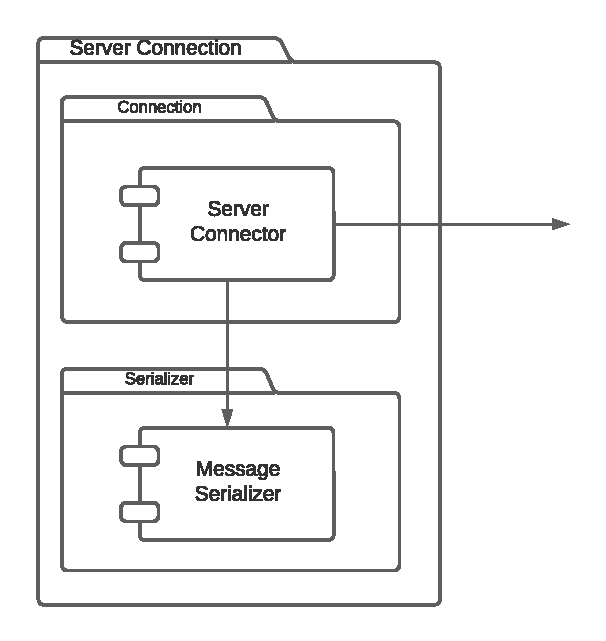
\includegraphics[scale=.65,center]{medien/server-connection.pdf}
    \caption{Server Connection}
    \ownsource
    \label{fig:server-connection}
\end{figure}

% \FloatBarrier

Er verwendet den gleich konfigurierten Serialisierer wie das TRISS Backend und verbindet sich mit diesem über das WebSocket Protokoll.
Das erlaubt es dem Backend, Frames zum Client zu übertragen, ohne dass dieser diese erst anfragen muss und automatisch über Änderungen am Server informiert wird, wie beispielweise, dass ein neuer Agent erstellt worden ist.

Diese Informationen leitet er via Actions an den Redux Store weiter.
Angesprochen wird er durch Reducer, die bei bestimmten Actions Anfragen an das Backend senden wollen.

\subsubsection{Realm Component – UI and Interactivity}

Die Komponente UI and Interactivity umfasst primär die React Komponenten.
Dadurch ist für diese React\footnote{\url{https://reactjs.org/}} die tragende Technologie.
Mit ihr lassen sich Funktionen definieren, die als Abbildungsfunktionen aufgefasst werden können, die einen konkreten Zustand in einen (Teil-)DOM übertragen.

Ein großer Vorteil von React ist, dass man die Benutzeransicht in einzelne deklarative Komponenten aufteilt, die man für sich genommen entwickeln und testen kann.
Übergeordnete Komponenten verwenden dann untergeordnete auf die gleiche Art und Weise wie man auch native HTML-Elemente gebrauchen würde.
Hinzu kommt das React durch den JSX bzw. TSX Syntax eine ausgesprochen übersichtliche programmierung erlaubt.

\begin{figure}[htb]
    \centering
    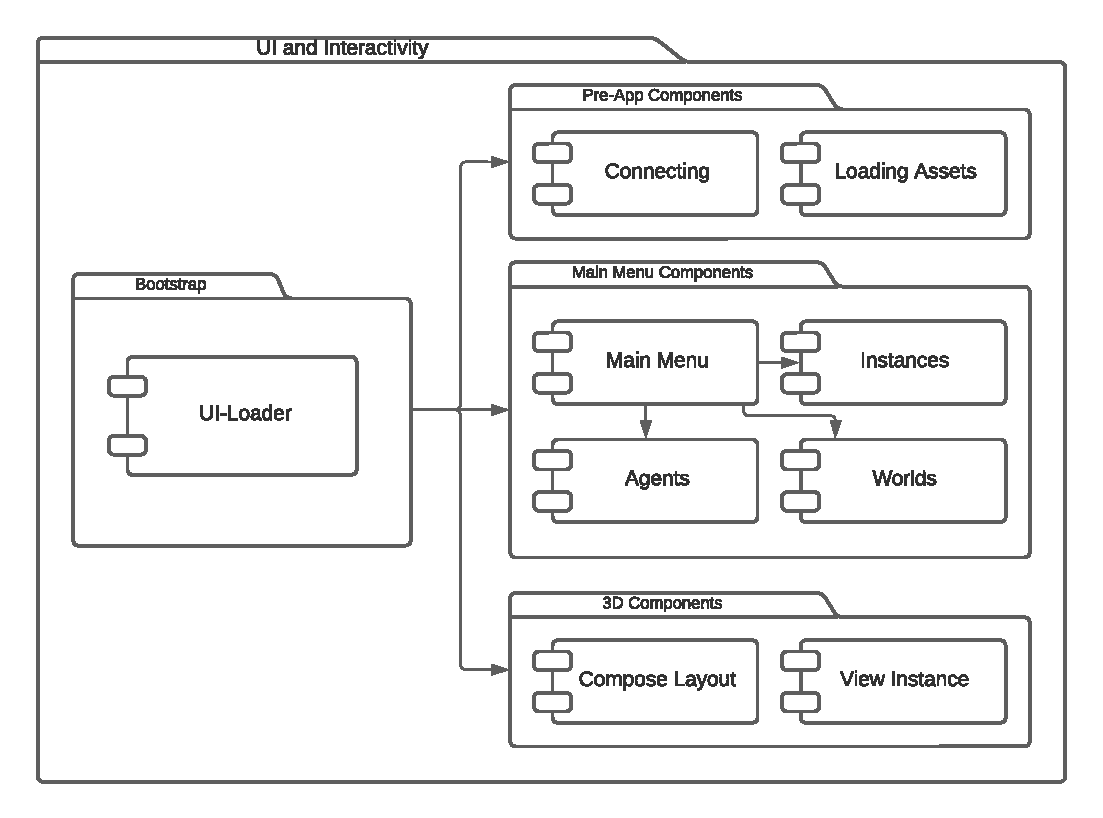
\includegraphics[scale=.65,center]{medien/ui-and-interactivity.pdf}
    \caption{UI and Interactivity}
    \ownsource
    \label{fig:ui-and-interactivity}
\end{figure}

% \FloatBarrier

Die Komponenten sind für die Darstelung in drei Gruppen unterteilt, welche ihren jeweiligen Schwerpunkt repräsentieren.
Zusammengebracht werden sie vom UI-Loader, der durch den im Store hinterlegten Pfad entscheidet, welche Komponenten aktuell geladen werden sollen.
Diese hängt er dann im DOM ein.
Dadurch rendert dann React diese Komponenten, wodurch dann via den React Hooks\footnote{\url{https://reactjs.org/docs/hooks-intro.html}} der aktuelle Zustand aus dem Redux Store gelesen wird und der Komponente zur Verfügung steht.

Diese erzeugt dann daraus den Pseudo DOM, der React mit dem realen abgleicht und wenn notwendig synchronisiert.
Nutzerinteraktionen werden via Events der Komponenten gemeldet, die diese in eine Action umwandelt und diese an den Store weitergibt.
Dieser verarbeitet dann, wie bereits beschrieben, diese Action mit Reducern, wodurch sich mit hoher Wahrscheinlichkeit der Zustand des Stores ändert und dadurch React die UI neu erzeugt.

Diese Komponenten haben also selbst keinen Zustand sondern spiegeln immer nur den Zustand wider, der im Redux Store enthalten ist.
Für die 3D-Components gilt zusätzlich das sie nur das UI für die 3D-Darstellung liefern, die 3D-Darstellung allerdings nicht übernehmen, sondern nur die DOM-Komponente für das Rendering in den DOM hängen.

\subsubsection{Realm Component – 3D Rendering}

Der 3D-Renderer ist das Herzstück des Frontends und hauptsächlich dafür verantwortlich, die von dem Server übertragenen Entitäten anschaulich darzustellen.
Um dies zu ermöglichen, wird hier sehr zentral mit der WebGL Schnittstelle des Browsers über die Bibliothek three.js gearbeitet.

Die Rendering Architektur ist dabei als Pipeline aufgebaut, da die Entitäten für die Darstellung mehrmals erweitert, zusammengefasst und gefiltert werden müssen.
Der Pipeline-Ansatz erlaubt es auch, neue Schritte einfach einzufügen und ganze Gruppen von Objekten zwischenzuspeichern, sollte sich herausstellen, dass sich die Eingabedaten in diesem Schritt nicht geändert haben.

So können neue Daten einfach am Anfang der Pipeline angelegt werden und die Änderungen kaskadieren dann bis zur eigentlichen Szenebildung mit Objekten, die three.js wiederum in Speicherstrukturen umformt, die durch WebGL verarbeitet werden können.

Zusätzlich erlaubt diese Struktur es, diese 3D-Darstellung in Zukunft einfacher zu parallelisieren,
auch wenn dafür vorher sichergestellt werden muss, dass der Overhead der De-/Serialisierung der Daten nicht größer ist als die eigentliche Umformung.

\begin{figure}[htb]
    \centering
    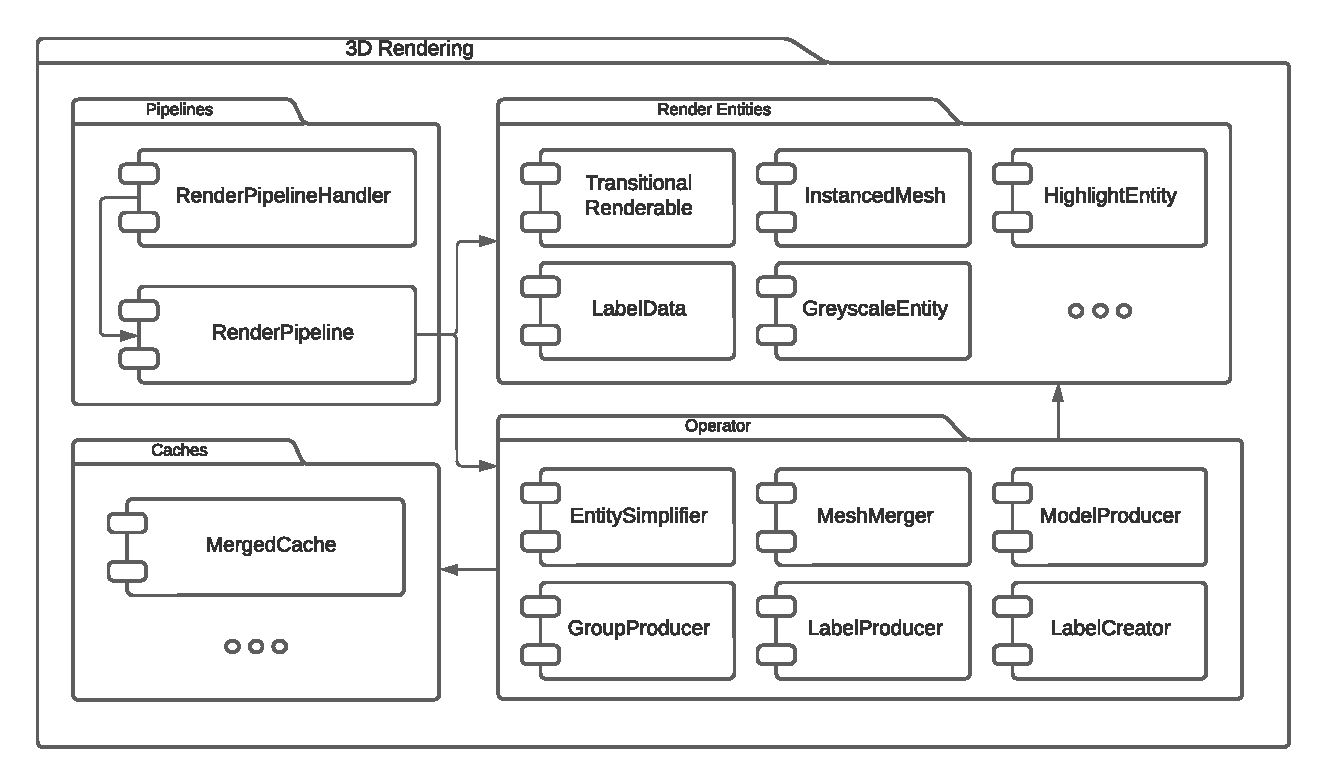
\includegraphics[scale=.65,center]{medien/3d-rendering.pdf}
    \caption{3D Rendering}
    \ownsource
    \label{fig:3d-rendering}
\end{figure}

% \FloatBarrier

Die 3D-Darstellung teilt sich dabei konkret in vier Pakete auf.
Das Operator Paket ist dabei das, das die eigentliche Funktionalität ermöglicht, indem es atomare Aktionen der Verarbeitung bereitstellt.
Diese Schritte umfassen Aufgaben, bei denen aus einer oder mehreren Eingabemengen eine oder mehrere Ausgabemengen erzeugt werden.

Beispielweise wird durch den Entity Simplifier aus der Positionsangabe, seiner Rotation und dem Typen der Entität das eigentliche 3D-Modell geladen bzw. erzeugt
und die Welt-Matrix berechnet, die seine Position widerspiegelt.

Der Mesh Merger hingegen ist dafür zuständig, aus einer Menge von Transitional Renderable Objekten Instanced Meshes zu erzeugen, die vom Shader Programm, das three.js bereitstellt, verarbeitet werden können und besonders effizient sind.

Alle Operatoren greifen dabei auf unterschiedlichste, auch teilweise verkettete Caches zu.
Diese Caches erlauben die Wiederverwendung von bereits erzeugten Objekten bzw. deren konkreten Konfigurationen.

Als Beispiel ist hier der Marked Cache anzuführen, der sich vor allem dadurch auszeichnet, dass er Einträge markiert, die in diesem Renderzyklus noch nicht verwendet worden sind.
Das erlaubt es, den Cache auch wieder zu entleeren, sodass dieser auch bei langanhaltender Verwendung nicht vollläuft und die Anwendung zum Absturz bringt.

Die Operatoren werden jedoch nicht direkt verwendet, da sie so noch keinen Nutzen haben.
Ihre eigentliche semantische Funktionalität wird erst durch die Render Pipeline erzeugt.
Diese nutzt die atomaren Operatoren, verknüpft sie und definiert, welche Daten in welchen Operator und in welchem Schritt geleitet werden sollen.

Diese Pipeline ist dafür gedacht, die dynamischen Entitäten, die durch den Agenten bzw. den Server definiert werde, in ihre respektiven (Teil-)Szenen\-graphen zu überführen.
Dies allein reicht jedoch nicht aus, um sie darstellen und mit ihnen interagieren zu können.
Diesen Anteil stellt der RenderPipelineHandler bereit.
Dieser erzeugt neben der Bodenplatte, dem Sonnenlicht und dem Firmament auch die Controller, die Nutzereingaben wie panning, zoom und click ermöglichen.

Zusätzlich macht er es sehr einfach, den Zustand der Welt zu aktualisieren.
Er ist die primäre und im Rahmen dieser Anwendung die einzige Komponente, die außerhalb des 3D-Moduls verwendet wird.
